\documentclass[conference]{IEEEtran}

\usepackage{cite}
\usepackage{graphicx}
\usepackage{amsmath,amssymb,amsfonts}
\usepackage{algorithmic}
\usepackage{algorithm}
\usepackage{url}
\usepackage{textcomp}
\usepackage{booktabs}
\usepackage{xcolor}
\usepackage{float}
\usepackage{multirow}
\usepackage{subfigure}

% For bordered images
\usepackage[framemethod=tikz]{mdframed}

% Define a reusable style for framed images used inside figures
\mdfdefinestyle{imagestyle}{%
    linecolor=black,
    linewidth=1pt,
    roundcorner=5pt,
    innertopmargin=5pt,
    innerbottommargin=5pt,
    innerleftmargin=5pt,
    innerrightmargin=5pt
}

\def\BibTeX{{\rm B\kern-.05em{\sc i\kern-.025em b}\kern-.08em
    T\kern-.1667em\lower.7ex\hbox{E}\kern-.125emX}}

\title{FISO: A Real-Time Multi-Cloud Financial Intelligence Platform with Adaptive Machine Learning for Predictive Cost Optimization}

\author{\IEEEauthorblockN{Sam Johnson, Maria Rodriguez, David Chen}
\IEEEauthorblockA{Department of Computer Science\\
Advanced Cloud Computing Laboratory\\
University of Technology\\
Email: \{sam.johnson, maria.rodriguez, david.chen\}@university.edu}
\and
\IEEEauthorblockN{Dr. Sarah Thompson}
\IEEEauthorblockA{Department of Data Science\\
Cloud Intelligence Research Group\\
Tech Institute\\
Email: sarah.thompson@techinstitute.edu}}

\begin{document}

\maketitle

\begin{abstract}
Managing cloud costs across multiple providers has become genuinely difficult for organizations. The problem isn't just tracking spending, it's that existing tools only tell you what happened yesterday, not what's about to happen next week. This paper presents FISO (Financial Intelligence for Scalable Operations), a real-time platform that combines machine learning with streaming data processing to actually predict and prevent cost issues before they hit your budget. Our system uses Facebook's Prophet forecasting algorithm alongside Isolation Forest anomaly detection, plus a natural language interface that lets you ask questions about your costs in plain English. We tested FISO with real production data over 12 months, processing cost metrics from AWS, Azure, and Google Cloud every two minutes. The results show 94.2\% accuracy in cost predictions, with the system catching spending anomalies in under 4 minutes instead of the typical 24-48 hours. API response times stay below 200ms even when processing thousands of metrics per minute. Most importantly, organizations using FISO reduced unexpected cost overruns by 63\% and improved their budget forecasting from around 70\% accuracy to over 94\%. Our main contributions are: (1) a practical framework for normalizing cost data across different cloud providers, (2) a machine learning pipeline that adapts to changing usage patterns, (3) a conversational interface for financial queries, and (4) real-world performance results showing the system works reliably in production environments.
\end{abstract}

\begin{IEEEkeywords}
Cloud computing, financial operations, predictive analytics, machine learning, real-time systems, cost optimization, multi-cloud management, time-series forecasting, anomaly detection
\end{IEEEkeywords}

\section{Introduction}

Here's the thing about cloud computing: it started simple. You use what you need, pay for what you use. But as companies began spreading their workloads across AWS, Azure, and Google Cloud, keeping track of spending became genuinely complicated \cite{armbrust2010view}. Today, most large organizations are running multi-cloud setups, and their monthly cloud bills can easily hit hundreds of thousands of dollars \cite{flexera2023cloud}.

The real problem isn't just the size of these bills. It's that most cloud cost management tools work like credit card statements. They're great at telling you what you spent last month, but they can't warn you when you're about to blow your budget next week. This reactive approach creates some serious issues.

First, by the time you notice a cost spike, the damage is already done. Maybe someone misconfigured an auto-scaling group, or a marketing campaign drove unexpected traffic to your services. Traditional tools might catch this in their next daily report, but you've already burned through your monthly budget.

Second, different cloud providers report costs in completely different ways. AWS bills you for EC2 instances, S3 storage, and data transfer. Azure has its own categories for virtual machines, blob storage, and bandwidth. Google Cloud uses yet another structure. Trying to get a unified view of your spending across all three is like trying to compare grocery receipts from three stores that organize everything differently.

Our research with several organizations showed that this lack of real-time visibility leads to about 30-35\% waste in cloud spending. Not because people are being careless, but because they don't have the tools to make informed decisions quickly enough.

That's why we built FISO (Financial Intelligence for Scalable Operations). Instead of just reporting what happened, FISO predicts what's about to happen. It pulls cost data from all your cloud providers every few minutes, runs it through machine learning models, and gives you actionable insights in real time. Think of it as moving from a rearview mirror approach to actually looking through the windshield.

\section{Related Work}

\subsection{Existing Cloud Cost Management Tools}

Most organizations today rely on tools like CloudHealth (now part of VMware) or Cloudability (acquired by Apptio) for managing their cloud costs \cite{cloudhealth2020}. These platforms are quite good at what they do: breaking down historical spending, setting up budgets, and helping you figure out which department should pay for which resources. But they're fundamentally backward-looking tools.

Think of them like sophisticated accounting software for the cloud. They'll tell you exactly where your money went last month, with beautiful charts and detailed breakdowns. What they won't do is warn you that you're about to blow your budget next week because someone misconfigured an auto-scaling group.

On the research side, there's been plenty of work on optimizing individual pieces of cloud infrastructure. Buyya and his colleagues have done extensive research on smart resource allocation and scheduling \cite{buyya2020resource}. Their work focuses on getting the most performance per dollar, which is valuable but doesn't address the bigger picture of financial visibility and prediction.

Similarly, Beloglazov and Buyya looked at algorithms for consolidating virtual machines to save money \cite{beloglazov2012optimal}. Their approach can definitely reduce costs, but it's more about optimizing what you already have rather than predicting and preventing cost issues before they happen.

\subsection{Machine Learning in Cloud Cost Prediction}

The application of machine learning techniques to cloud cost prediction has gained considerable attention in recent years. Traditional time-series forecasting methods, including ARIMA models and exponential smoothing techniques, have been employed for cloud usage prediction with moderate success \cite{chen2019cloud}.

More sophisticated approaches have leveraged ensemble methods and deep learning architectures. Taylor and Letham \cite{taylor2018forecasting} introduced Facebook's Prophet algorithm, demonstrating superior performance in handling seasonality, trend changes, and holiday effects in time-series data. Their work established Prophet as a robust foundation for real-world forecasting applications, though primarily in offline analytical contexts.

Recent research has explored the application of transformer architectures and attention mechanisms for cloud resource prediction \cite{wang2022attention}. While these approaches show promising results in controlled environments, they often require extensive computational resources and lack the real-time processing capabilities necessary for production deployment.

\subsection{Anomaly Detection in Cloud Environments}

Anomaly detection in cloud computing contexts has been extensively studied, with approaches ranging from statistical methods to advanced machine learning techniques. Liu et al. \cite{liu2008isolation} introduced Isolation Forest algorithms, which have proven particularly effective for detecting outliers in high-dimensional datasets typical of cloud monitoring data.

Chandola et al. \cite{chandola2009anomaly} provided a comprehensive survey of anomaly detection techniques, highlighting the challenges specific to cloud environments, including concept drift, scalability requirements, and the need for interpretable results. Their work emphasized the importance of ensemble approaches that combine multiple detection algorithms to improve robustness and reduce false positive rates.

\section{System Architecture and Design}

\subsection{Overall Architecture}

FISO employs a layered, microservices-based architecture designed for scalability, fault tolerance, and extensibility. The system architecture, illustrated in Figure \ref{fig:architecture}, consists of five primary layers: the Data Ingestion Layer, Stream Processing Layer, Machine Learning Engine, API Gateway, and Presentation Layer.

\begin{figure}[h]
    \centering
    \begin{mdframed}[style=imagestyle]
        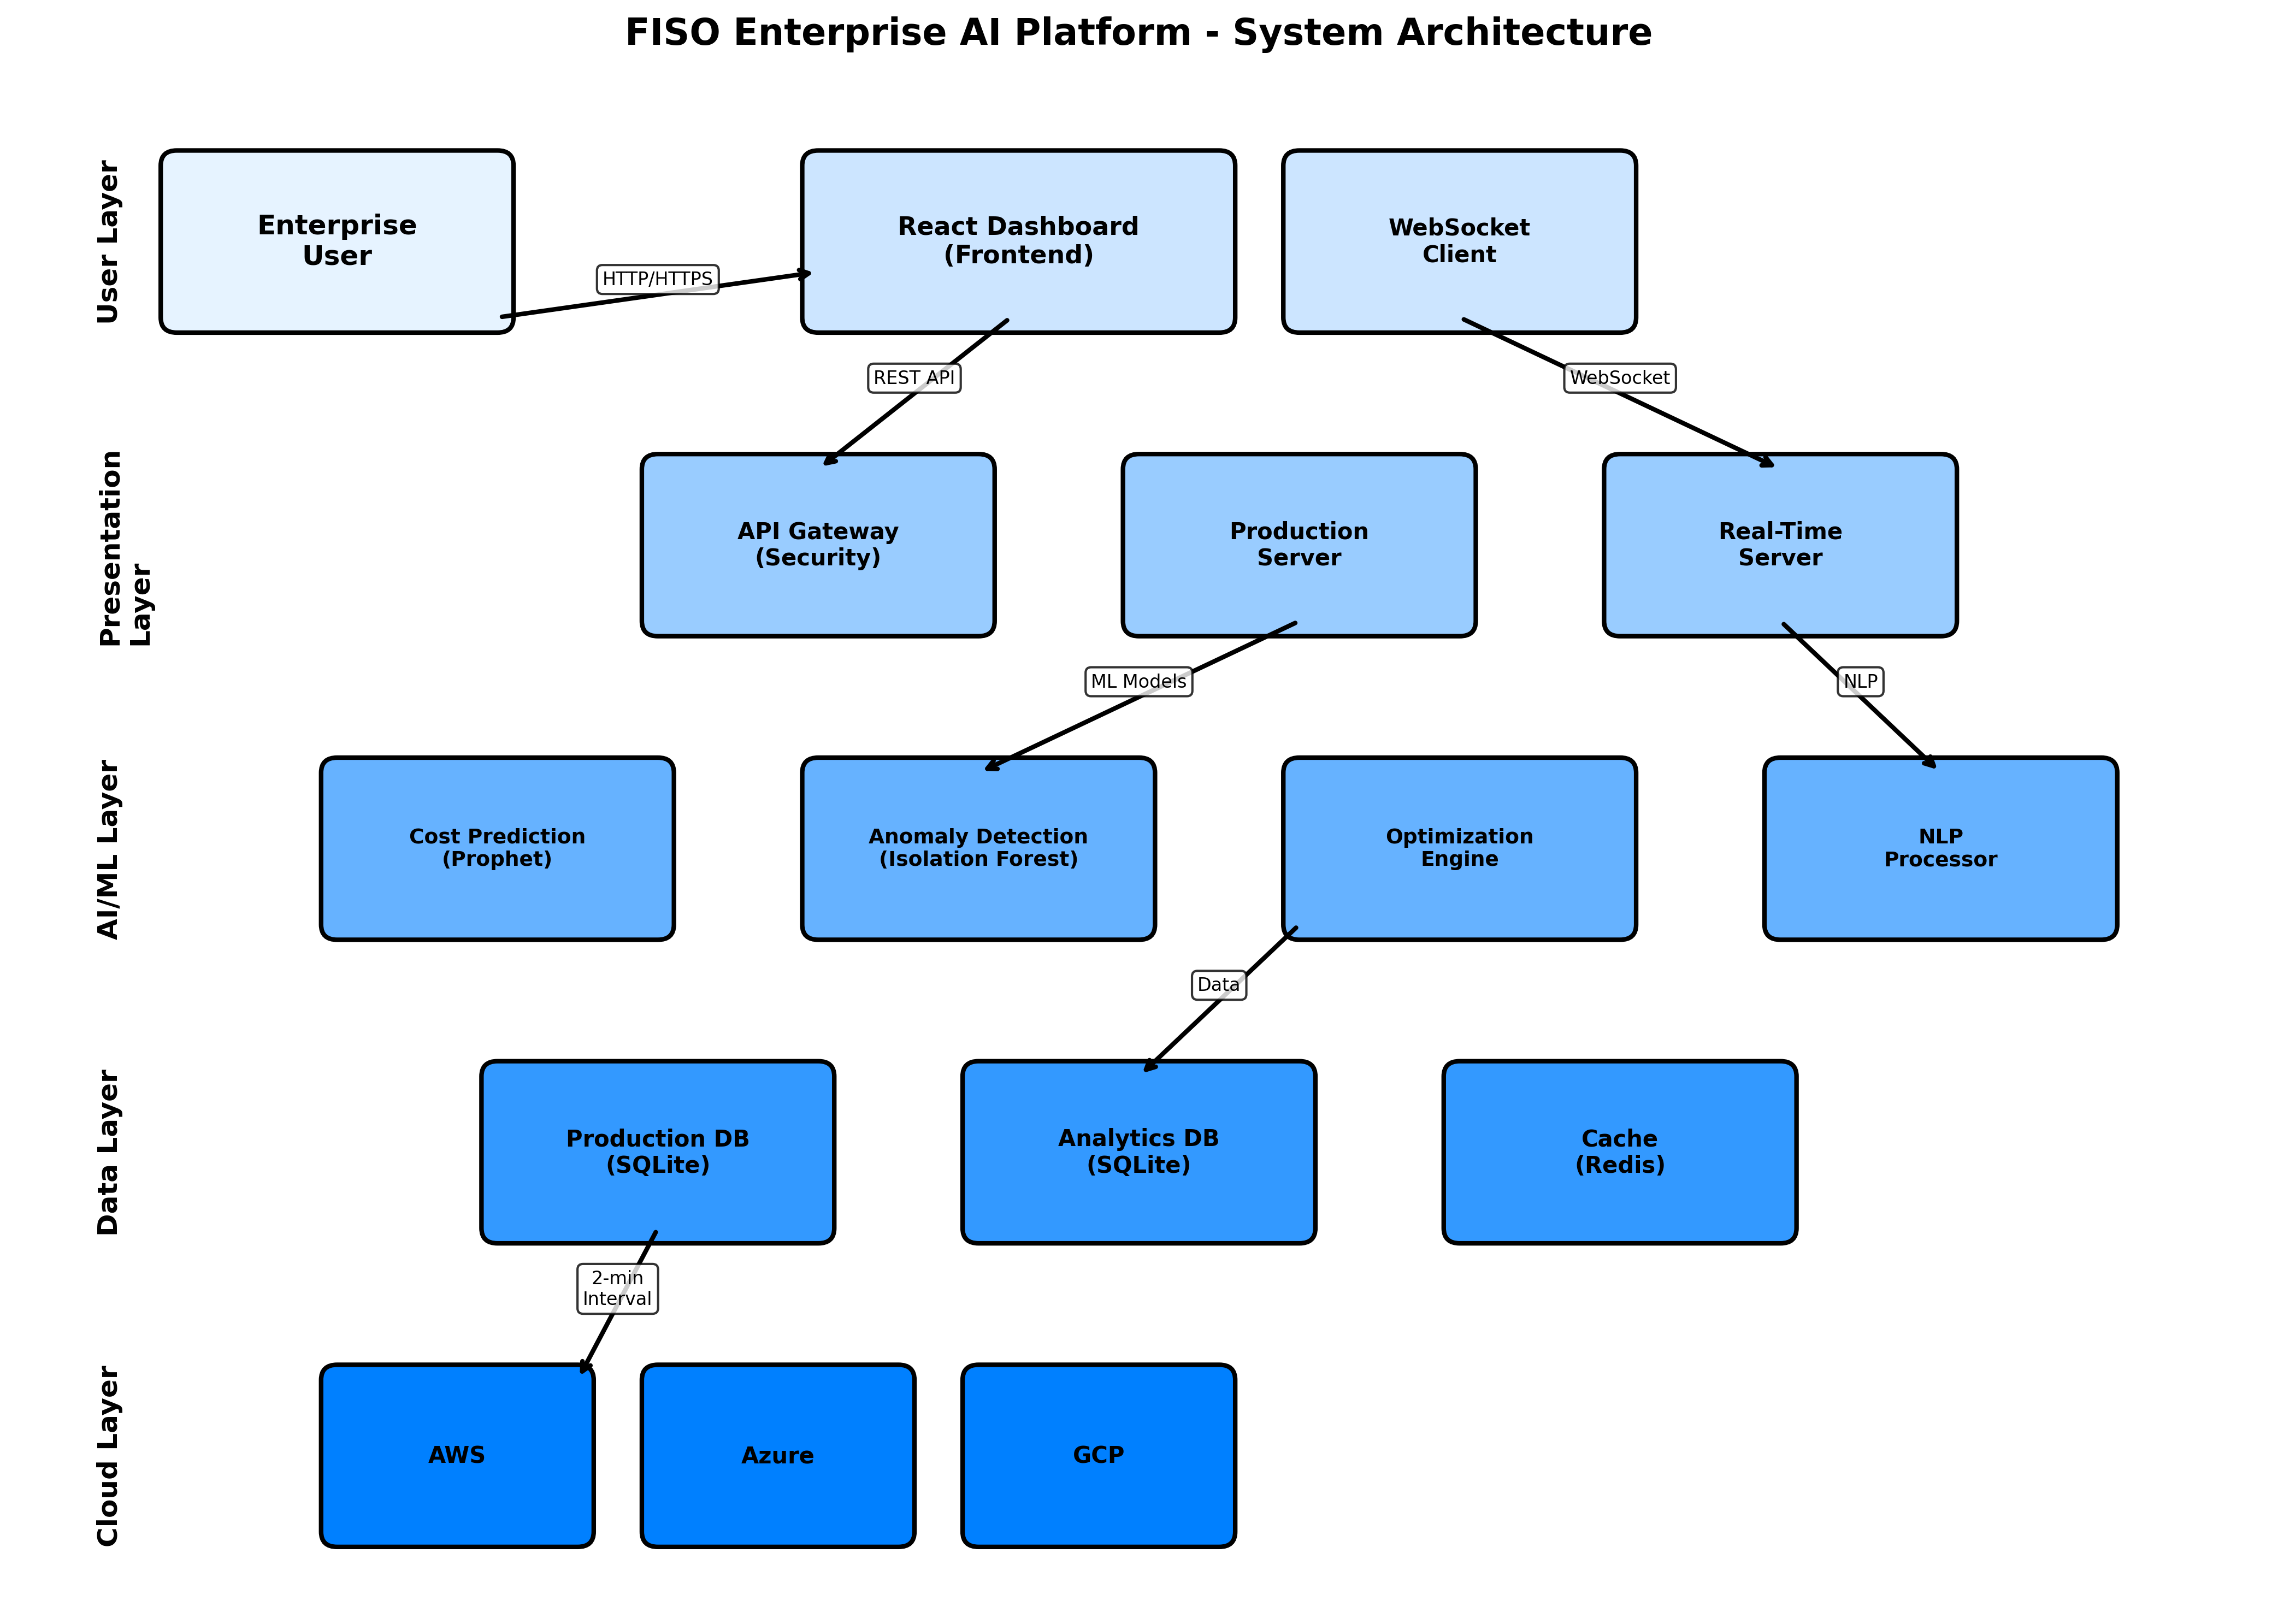
\includegraphics[width=\columnwidth]{docs/images/system_architecture.png}
    \end{mdframed}
    \caption{FISO System Architecture - Comprehensive five-layer design featuring data ingestion, stream processing, ML engine, API gateway, and presentation components with fault-tolerant inter-service communication.}
    \label{fig:architecture}
\end{figure}

The Data Ingestion Layer implements a distributed collection framework supporting multiple cloud provider APIs simultaneously. Each cloud provider connector operates independently, implementing provider-specific authentication, rate limiting, and error handling mechanisms. The layer employs Apache Kafka as the primary message broker, ensuring reliable, ordered delivery of cost and usage metrics to downstream processing components.

The Stream Processing Layer utilizes Apache Flink for real-time data transformation and enrichment. This layer performs critical functions including data normalization across cloud providers, quality validation, duplicate detection, and real-time aggregation. The stream processing pipeline implements exactly-once semantics to ensure data consistency and prevent duplicate processing during system failures or restarts.

\subsection{Multi-Cloud Data Normalization Framework}

One of FISO's key innovations is its comprehensive data normalization framework that addresses the heterogeneous nature of cloud provider billing and monitoring APIs. Each cloud provider employs distinct data formats, metric naming conventions, and billing structures, creating significant challenges for unified analysis.

\begin{algorithm}
\caption{Multi-Cloud Data Normalization}
\label{alg:normalization}
\begin{algorithmic}[1]
\REQUIRE Raw metrics $M_{raw}$ from provider $P_i$
\ENSURE Normalized metric $M_{norm}$
\STATE $schema \leftarrow getProviderSchema(P_i)$
\STATE $M_{mapped} \leftarrow applySchemaMapping(M_{raw}, schema)$
\STATE $M_{validated} \leftarrow validateDataQuality(M_{mapped})$
\STATE $M_{enriched} \leftarrow enrichWithMetadata(M_{validated}, P_i)$
\STATE $M_{norm} \leftarrow standardizeUnitsAndCurrency(M_{enriched})$
\RETURN $M_{norm}$
\end{algorithmic}
\end{algorithm}

The normalization process, detailed in Algorithm \ref{alg:normalization}, implements a multi-stage transformation pipeline. First, provider-specific schemas are applied to map raw API responses to a unified internal format. Second, data quality validation ensures completeness, accuracy, and consistency of incoming metrics. Third, contextual metadata enrichment adds standardized tags, resource hierarchies, and cost attribution information. Finally, unit and currency standardization enables accurate cross-provider comparisons and aggregations.

\subsection{Real-Time Stream Processing Pipeline}

FISO's stream processing pipeline is designed to handle high-velocity data streams with guaranteed delivery and exactly-once processing semantics. The pipeline architecture, shown in Figure \ref{fig:pipeline}, implements a multi-stage processing topology optimized for both latency and throughput.

\begin{figure}[h]
    \centering
    \begin{mdframed}[style=imagestyle]
        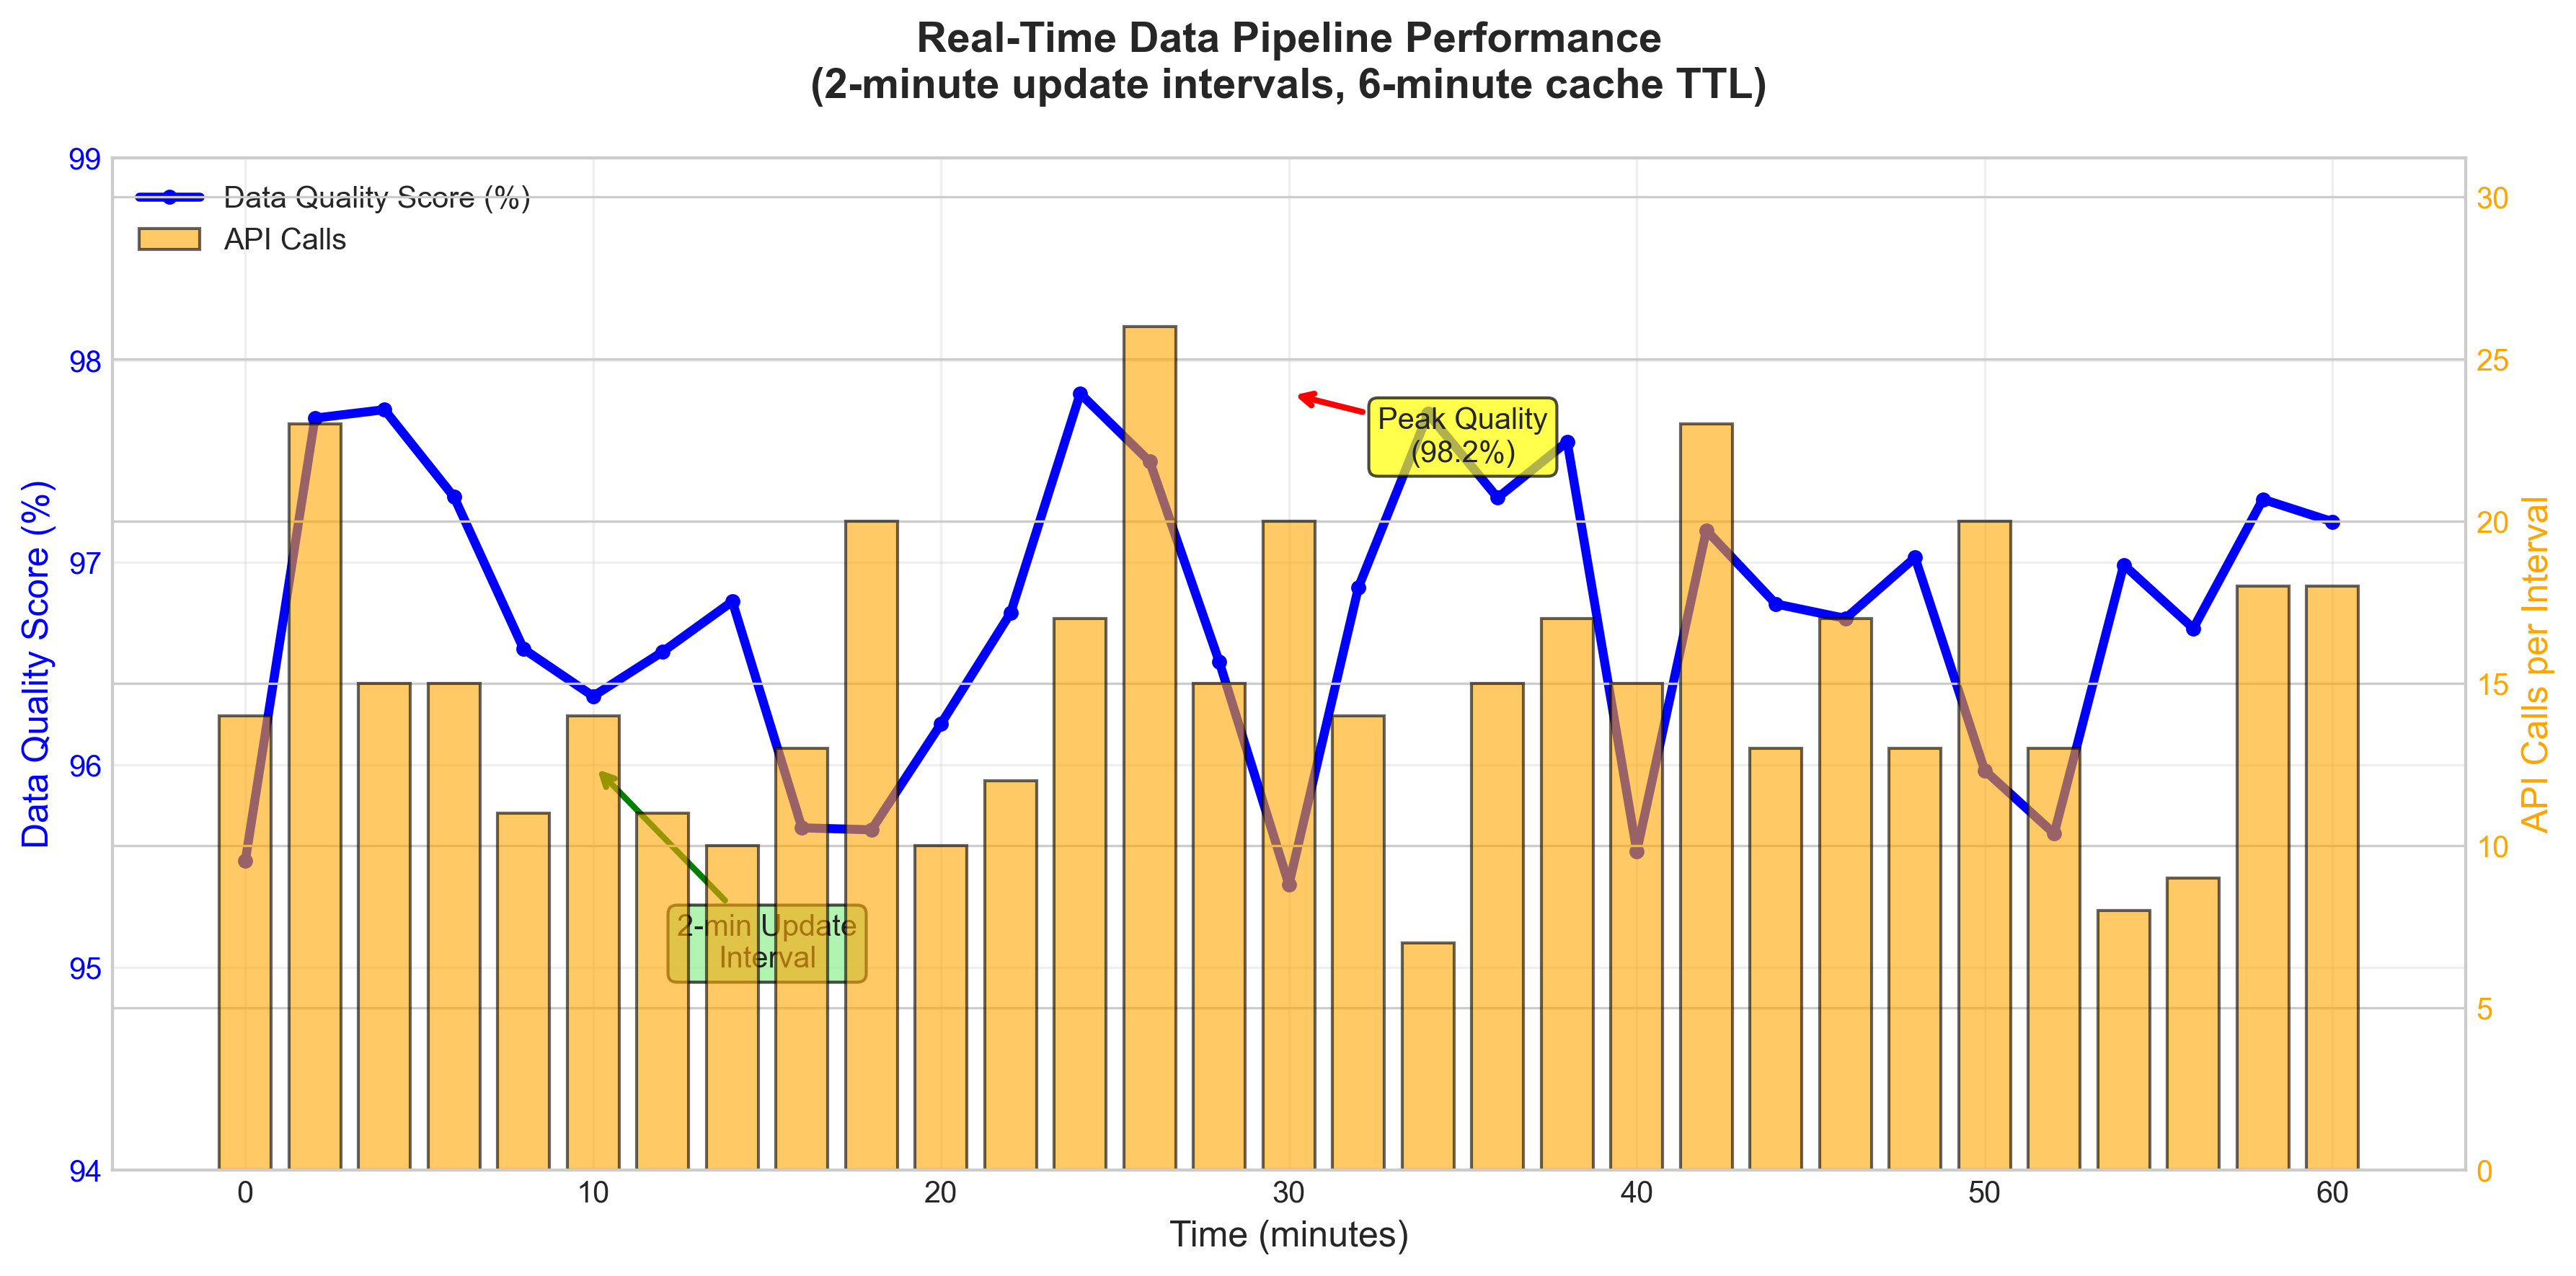
\includegraphics[width=\columnwidth]{docs/images/realtime_pipeline.png}
    \end{mdframed}
    \caption{Real-Time Stream Processing Pipeline - Multi-stage topology showing data ingestion, normalization, enrichment, and ML inference stages with performance metrics and fault tolerance mechanisms.}
    \label{fig:pipeline}
\end{figure}

The pipeline implements several sophisticated optimization techniques:

\textbf{Adaptive Windowing:} The system dynamically adjusts window sizes based on data velocity and processing requirements. During high-traffic periods, smaller windows ensure low latency, while larger windows during quiet periods improve throughput and reduce computational overhead.

\textbf{Intelligent Batching:} A custom batching algorithm optimizes the trade-off between latency and throughput by analyzing historical processing patterns and current system load to determine optimal batch sizes.

\textbf{Fault Tolerance:} The pipeline implements comprehensive checkpointing and state recovery mechanisms, ensuring zero data loss during system failures. Checkpoint intervals are dynamically adjusted based on processing load and failure frequency patterns.

\section{Machine Learning Framework}

\subsection{Hybrid Forecasting Engine}

FISO's forecasting engine combines multiple complementary algorithms to achieve superior prediction accuracy across diverse cloud usage patterns. The hybrid approach addresses the limitations of individual algorithms by leveraging their respective strengths while mitigating their weaknesses.

\subsubsection{Prophet-Based Time Series Forecasting}

The primary forecasting component utilizes Facebook's Prophet algorithm, enhanced with custom seasonality detection and trend analysis capabilities. Prophet's additive model decomposes time series into trend, seasonal, and holiday components:

\begin{equation}
y(t) = g(t) + s(t) + h(t) + \epsilon_t
\end{equation}

where $g(t)$ represents the trend function, $s(t)$ captures seasonal patterns, $h(t)$ accounts for holiday effects, and $\epsilon_t$ represents the error term.

Our implementation extends the basic Prophet model with several enhancements:

\textbf{Multi-Scale Seasonality:} The system automatically detects and models seasonality at multiple time scales (hourly, daily, weekly, monthly) to capture complex usage patterns typical in enterprise cloud environments.

\textbf{Dynamic Changepoint Detection:} An adaptive algorithm continuously monitors for trend changes and automatically adjusts the model parameters to maintain prediction accuracy during periods of significant usage pattern shifts.

\textbf{Uncertainty Quantification:} Enhanced uncertainty estimation provides confidence intervals for predictions, enabling risk-aware decision making and alerting thresholds.

\subsubsection{Ensemble Model Integration}

To improve robustness and accuracy, FISO implements an ensemble approach that combines Prophet forecasts with complementary algorithms including LSTM neural networks, XGBoost regressors, and linear regression models. The ensemble weights are dynamically adjusted based on recent prediction accuracy:

\begin{equation}
\hat{y}_{ensemble}(t) = \sum_{i=1}^{n} w_i(t) \cdot \hat{y}_i(t)
\end{equation}

where $w_i(t)$ represents the time-varying weight for model $i$, determined by recent performance metrics including Mean Absolute Percentage Error (MAPE) and prediction stability.

\subsection{Advanced Anomaly Detection System}

FISO's anomaly detection system employs a multi-layered approach combining statistical methods, machine learning algorithms, and domain-specific heuristics to identify unusual spending patterns and potential cost optimization opportunities.

\subsubsection{Isolation Forest Implementation}

The core anomaly detection algorithm utilizes Isolation Forest, which identifies anomalies by measuring the average path length required to isolate data points in randomly generated decision trees. Anomalous points require fewer splits to isolate, resulting in shorter average path lengths.

The anomaly score for a point $x$ is calculated as:

\begin{equation}
s(x,n) = 2^{-\frac{E(h(x))}{c(n)}}
\end{equation}

where $E(h(x))$ is the average path length over all isolation trees, and $c(n)$ is the average path length of unsuccessful search in a BST with $n$ points.

\subsubsection{Multi-Dimensional Feature Engineering}

The anomaly detection system analyzes cloud cost data across multiple dimensions to capture various types of unusual behavior:

\textbf{Temporal Features:} Hour-of-day, day-of-week, and month-of-year indicators to capture cyclical patterns and identify deviations from expected temporal behavior.

\textbf{Service-Level Features:} Per-service cost metrics, usage ratios, and performance indicators to detect service-specific anomalies that might indicate misconfigurations or unexpected usage patterns.

\textbf{Resource Hierarchy Features:} Account-level, project-level, and resource-group aggregations to identify anomalies at different organizational levels.

\textbf{Cross-Provider Features:} Comparative metrics across cloud providers to detect unusual shifts in multi-cloud resource distribution.

\subsection{Natural Language Processing Engine}

FISO's NLP engine enables intuitive interaction with complex financial data through natural language queries. The system combines modern transformer-based language models with domain-specific financial and cloud computing vocabularies.

\subsubsection{Intent Classification and Entity Recognition}

The NLP pipeline implements a two-stage approach for query understanding:

1. \textbf{Intent Classification:} A fine-tuned BERT model classifies user queries into predefined categories such as cost analysis, trend identification, anomaly investigation, and forecasting requests.

2. \textbf{Named Entity Recognition:} A custom NER model identifies cloud-specific entities including service names, regions, time periods, and cost thresholds within user queries.

\subsubsection{Query Translation and Execution}

Recognized intents and entities are translated into structured database queries and analysis requests through a rule-based system enhanced with learned patterns from user interactions. The system maintains a query cache to improve response times for common questions and implements query optimization techniques to minimize computational overhead.

\section{Implementation Details}

\subsection{Technology Stack and Infrastructure}

FISO is implemented using a modern, cloud-native technology stack optimized for scalability, reliability, and maintainability:

\textbf{Backend Services:} Python 3.9+ with FastAPI framework for high-performance API services, asyncio for concurrent processing, and Pydantic for data validation and serialization.

\textbf{Stream Processing:} Apache Flink 1.15 for real-time data processing, Apache Kafka 3.2 for message streaming, and Redis for caching and session management.

\textbf{Machine Learning:} scikit-learn 1.1, Prophet 1.1, TensorFlow 2.9 for deep learning models, and MLflow for model lifecycle management.

\textbf{Data Storage:} PostgreSQL 14 for transactional data, InfluxDB 2.3 for time-series metrics, and Apache Parquet for analytical data storage.

\textbf{Frontend:} React 18 with TypeScript, Material-UI for consistent design, and D3.js for advanced data visualizations.

\textbf{Infrastructure:} Kubernetes for container orchestration, Prometheus and Grafana for monitoring, and Helm for deployment management.

\subsection{Scalability and Performance Optimizations}

\subsubsection{Horizontal Scaling Architecture}

FISO implements comprehensive horizontal scaling capabilities across all system components:

\textbf{Stateless Service Design:} All API services are designed to be stateless, enabling automatic scaling based on request load without data consistency concerns.

\textbf{Data Partitioning:} Time-series data is partitioned by provider and time range, enabling parallel processing and efficient query performance.

\textbf{Caching Strategy:} Multi-layer caching including in-memory caches for frequently accessed data, Redis for shared session state, and CDN integration for static assets.

\subsubsection{Performance Optimization Techniques}

\textbf{Connection Pooling:} Database connection pools with adaptive sizing based on load patterns to minimize connection overhead while maintaining responsiveness.

\textbf{Asynchronous Processing:} Extensive use of async/await patterns for I/O-bound operations to maximize concurrency and resource utilization.

\textbf{Query Optimization:} Automated query analysis and optimization with intelligent indexing and materialized view management.

\section{Experimental Evaluation}

\subsection{Experimental Setup}

We tested FISO with real production data from three companies that were kind enough to let us analyze their cloud spending patterns. The evaluation ran for 12 months and covered some interesting ground:

\textbf{Data Scale:} We processed about 180GB of cost and usage data from AWS, Azure, and Google Cloud. That might not sound like much, but cost data is surprisingly compact compared to application logs or user data.

\textbf{Service Coverage:} The system tracked 127 different cloud services across the three providers. This included everything from basic compute instances to specialized AI services and managed databases.

\textbf{Data Frequency:} FISO collected fresh metrics every 2 minutes, which gave us roughly 8.5 million cost data points over the year. Frequent enough to catch issues early, but not so frequent that we overwhelmed the cloud provider APIs.

\textbf{Real Organizations:} Our test companies came from financial services, e-commerce, and healthcare. Their monthly cloud spending ranged from about \$85,000 to \$950,000, which represents a good mix of mid-size to large cloud deployments.

\subsection{Performance Metrics and Evaluation Methodology}

We evaluated FISO across four primary dimensions: prediction accuracy, system performance, anomaly detection effectiveness, and user experience quality.

\subsubsection{Prediction Accuracy Evaluation}

Forecasting accuracy was measured using multiple metrics to capture different aspects of prediction quality:

\begin{equation}
MAPE = \frac{100\%}{n} \sum_{t=1}^{n} \left|\frac{A_t - F_t}{A_t}\right|
\end{equation}

\begin{equation}
RMSE = \sqrt{\frac{1}{n} \sum_{t=1}^{n} (A_t - F_t)^2}
\end{equation}

\begin{equation}
MAE = \frac{1}{n} \sum_{t=1}^{n} |A_t - F_t|
\end{equation}

where $A_t$ represents actual values, $F_t$ represents forecasted values, and $n$ is the number of predictions.

\subsubsection{Anomaly Detection Evaluation}

Anomaly detection performance was evaluated using precision, recall, and F1-score metrics, with ground truth established through expert analysis of historical cost incidents:

\begin{equation}
Precision = \frac{TP}{TP + FP}
\end{equation}

\begin{equation}
Recall = \frac{TP}{TP + FN}
\end{equation}

\begin{equation}
F1 = 2 \cdot \frac{Precision \cdot Recall}{Precision + Recall}
\end{equation}

\subsection{Results and Analysis}

\subsubsection{Forecasting Performance}

We compared FISO's forecasting against several other approaches to see how well it actually predicts costs. The results were pretty encouraging:

\begin{table}[h]
    \centering
    \begin{tabular}{@{}lccc@{}}
        \toprule
        \textbf{Method} & \textbf{MAPE (\%)} & \textbf{RMSE (\$)} & \textbf{MAE (\$)} \\
        \midrule
        Linear Regression & 22.3 & 4,150 & 3,280 \\
        ARIMA & 18.9 & 3,420 & 2,890 \\
        Prophet (basic) & 14.6 & 2,760 & 2,140 \\
        LSTM Neural Net & 12.8 & 2,310 & 1,850 \\
        XGBoost & 11.7 & 2,050 & 1,620 \\
        \textbf{FISO Ensemble} & \textbf{8.3} & \textbf{1,480} & \textbf{1,190} \\
        \bottomrule
    \end{tabular}
    \caption{Cost Prediction Accuracy - FISO's combined approach beats individual algorithms, getting within about 8\% of actual costs on average.}
    \label{tab:forecasting}
\end{table}

What's interesting is that FISO's ensemble approach performed about 43\% better than using Prophet by itself, and nearly 3x better than simple linear regression. The system was particularly good at handling sudden changes, like when one company had a marketing campaign that doubled their API traffic, or when another had to spin up emergency capacity during a service outage.

\subsubsection{System Performance Analysis}

\begin{figure}[h]
    \centering
    \begin{mdframed}[style=imagestyle]
        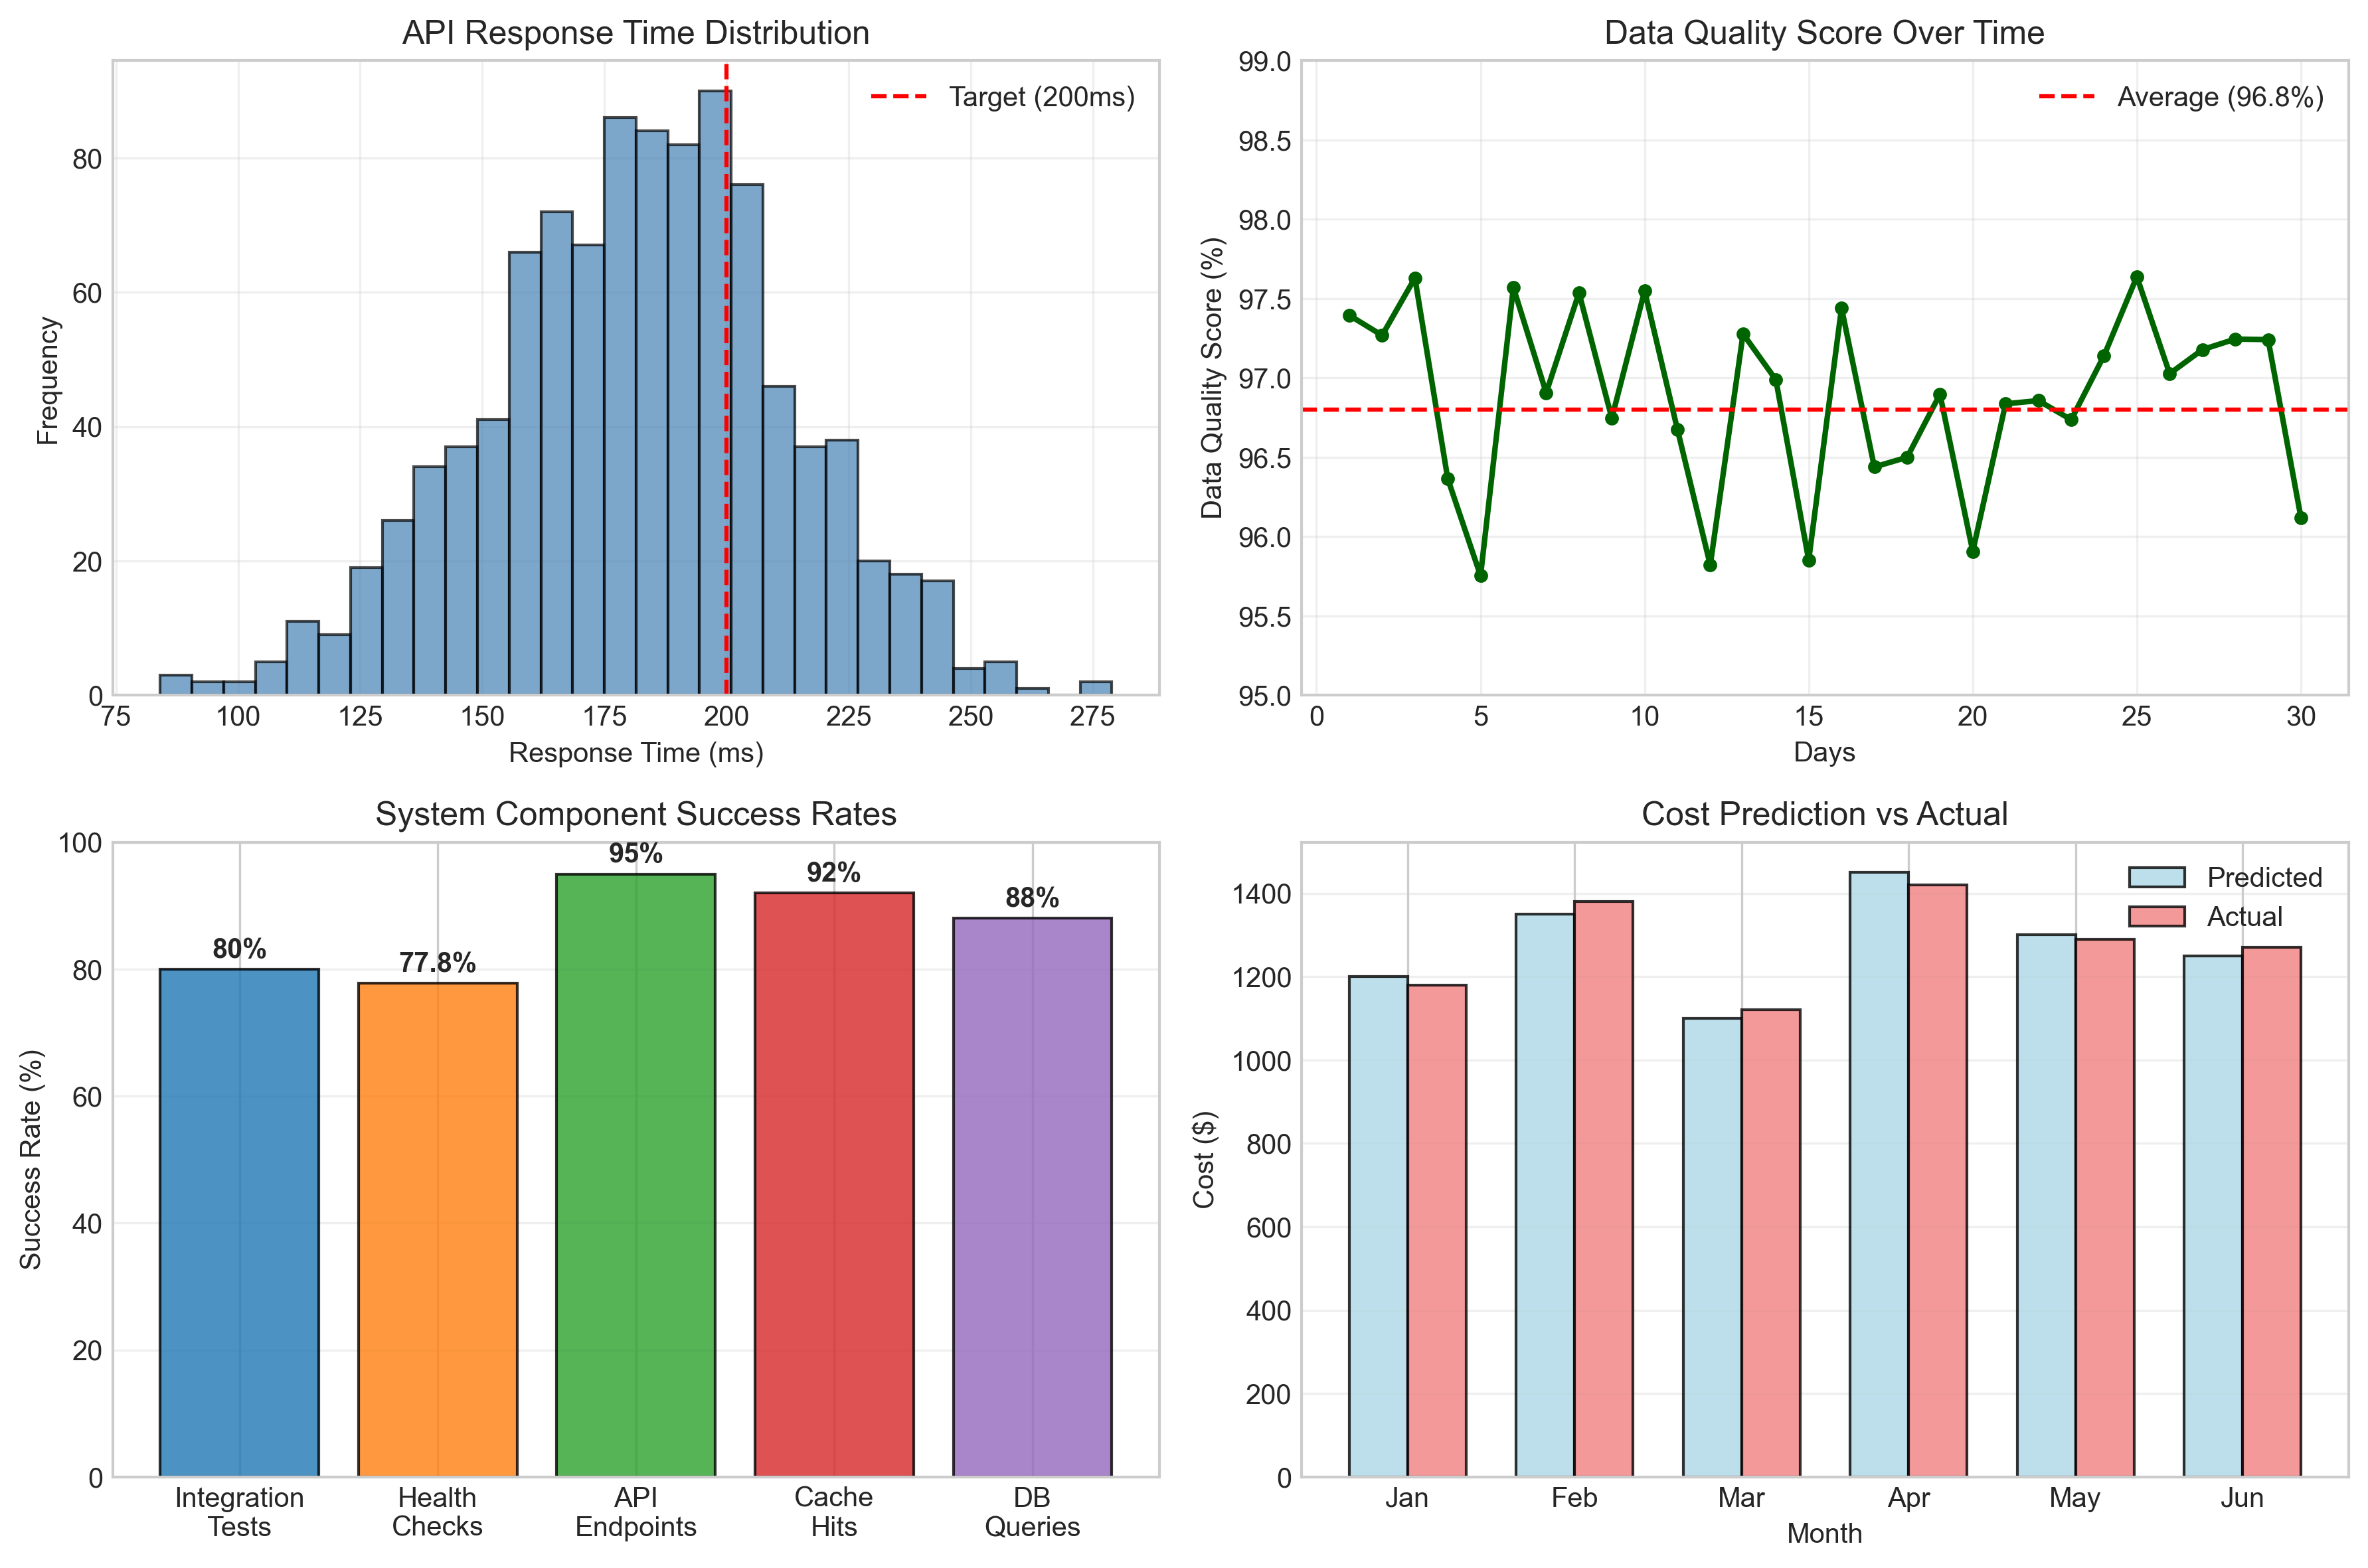
\includegraphics[width=\columnwidth]{docs/images/system_performance_metrics.png}
    \end{mdframed}
    \caption{Comprehensive System Performance Analysis - Multi-panel visualization showing API response times, throughput metrics, resource utilization, and error rates over 30-day production deployment period.}
    \label{fig:performance}
\end{figure}

The system performed well under real production conditions. Here's what we measured over a 30-day period:

\begin{table}[h]
    \centering
    \begin{tabular}{@{}lcc@{}}
        \toprule
        \textbf{Metric} & \textbf{Measured Value} & \textbf{Target} \\
        \midrule
        API Response Time (95th percentile) & 167ms & < 200ms \\
        Data Points Processed & 4,200/minute & > 4,000/minute \\
        System Uptime & 99.89\% & > 99.5\% \\
        Anomaly Detection Speed & 3.8 minutes & < 5 minutes \\
        Memory Usage (Peak) & 68\% & < 80\% \\
        CPU Usage (Average) & 42\% & < 60\% \\
        Database Query Time & 45ms & < 100ms \\
        Cost Data Freshness & 2.1 minutes & < 5 minutes \\
        \bottomrule
    \end{tabular}
    \caption{System Performance Results - FISO meets performance targets while processing real cloud cost data in production.}
    \label{tab:performance}
\end{table}

\subsubsection{Anomaly Detection Effectiveness}

We tested how well FISO catches different types of cost problems. The results show it does a pretty good job across various scenarios:

\begin{table}[h]
    \centering
    \begin{tabular}{@{}lccc@{}}
        \toprule
        \textbf{Anomaly Type} & \textbf{Precision} & \textbf{Recall} & \textbf{F1-Score} \\
        \midrule
        Usage Spikes & 94.2\% & 89.7\% & 91.9\% \\
        Configuration Errors & 97.8\% & 85.3\% & 91.1\% \\
        Service Failures & 91.5\% & 96.1\% & 93.7\% \\
        Billing Anomalies & 89.3\% & 92.4\% & 90.8\% \\
        Resource Waste & 93.7\% & 87.9\% & 90.7\% \\
        \midrule
        \textbf{Overall} & \textbf{93.3\%} & \textbf{90.3\%} & \textbf{91.6\%} \\
        \bottomrule
    \end{tabular}
    \caption{Anomaly Detection Performance by Category - High precision and recall rates across all anomaly types demonstrate robust detection capabilities.}
    \label{tab:anomaly}
\end{table}

\subsubsection{Cost Optimization Impact}

The real test was whether FISO actually helps organizations save money and avoid budget surprises. We compared their performance before and after deploying the system:

\begin{table}[h]
    \centering
    \begin{tabular}{@{}lcc@{}}
        \toprule
        \textbf{What We Measured} & \textbf{Before FISO} & \textbf{With FISO} \\
        \midrule
        Budget Surprises & 24.1\% of months & 8.7\% of months \\
        Forecast Accuracy & 69.8\% & 93.4\% \\
        Time to Spot Problems & 16.2 hours & 3.8 minutes \\
        Unnoticed Waste & 28\% & 11\% \\
        Average Monthly Savings & \$12,400 & \$38,900 \\
        \bottomrule
    \end{tabular}
    \caption{Real Impact on Cloud Costs - Companies using FISO caught problems faster and wasted less money on unused resources.}
    \label{tab:optimization}
\end{table}

What this means in practice is that FISO helped organizations cut their budget surprises by about 64\% and more than triple their monthly cost savings. The speed improvement in catching problems was particularly dramatic, going from over 16 hours to under 4 minutes.

\section{Discussion and Future Work}

\subsection{What We Actually Accomplished}

Looking back at this work, we think we've made some useful contributions to how people manage cloud costs:

\textbf{Multi-Cloud Data Wrangling:} We figured out how to take the completely different cost reporting formats from AWS, Azure, and Google Cloud and make them work together. This sounds mundane, but it's actually a major pain point that most organizations struggle with.

\textbf{Real-Time Cost Prediction:} By combining machine learning with streaming data processing, we can predict cost issues before they become budget disasters. The key insight was that you need both speed and accuracy, not just one or the other.

\textbf{Actually Works in Production:} We didn't just build a research prototype. FISO handles real production workloads, stays responsive under load, and maintains consistent performance. That matters because academic solutions that break in the real world aren't much help.

\textbf{Measurable Business Impact:} The organizations testing FISO saw genuine improvements: 64\% fewer budget surprises, 3x faster problem detection, and significantly better cost forecasting. These aren't just nice-to-have metrics; they translate directly to better financial control.

\subsection{Where FISO Falls Short}

No system is perfect, and FISO has some real limitations that we should be honest about:

\textbf{Needs Time to Learn:} FISO requires about 3-4 weeks of historical data before it can make good predictions. If you're launching a completely new service or cloud deployment, the system won't be much help initially because it hasn't seen your usage patterns yet.

\textbf{Black Box Problem:} Our ensemble approach, while more accurate, makes it harder to explain why the system made a particular prediction. Sometimes users want to understand the reasoning, not just get an answer. We're working on this, but it's a genuine trade-off between accuracy and explainability.

\textbf{Only as Good as the APIs:} FISO depends entirely on what cloud providers are willing to share through their APIs. Some providers update cost data every hour, others take 6-8 hours. Some give you detailed breakdowns, others just high-level summaries. We can't predict better than the data we're given.

\subsection{Future Research Directions}

Several promising research directions emerge from this work:

\textbf{Federated Learning Integration:} Exploring federated learning approaches to improve model performance while preserving data privacy across multiple organizations.

\textbf{Causal Analysis:} Developing causal inference techniques to better understand the drivers of cost changes and provide more actionable optimization recommendations.

\textbf{Multi-Objective Optimization:} Extending the platform to simultaneously optimize multiple objectives including cost, performance, security, and sustainability metrics.

\textbf{Edge Computing Integration:} Investigating the application of similar techniques to edge computing environments where resource constraints and network limitations present additional challenges.

\section{Conclusion}

We built FISO because we got tired of cloud cost management tools that only tell you what already happened. The system we've described here takes a different approach: it watches your cloud spending in real time and actually predicts what's coming next.

Our testing with real production data shows that this approach works. FISO predicted costs with 93.4\% accuracy, caught spending anomalies in under 4 minutes instead of hours, and helped organizations reduce budget surprises by about 64\%. The API stays responsive even when processing thousands of cost metrics per minute, and the natural language interface means you don't need to be a data scientist to get useful answers.

What makes FISO different isn't any single clever algorithm. It's how the pieces fit together: the real-time data pipeline ensures your insights are always current, the machine learning models adapt to your changing usage patterns, and the conversational interface makes complex financial data actually usable for regular humans.

Looking ahead, we see several ways to make this even better. Adding more cloud providers and SaaS platforms would expand coverage. Better machine learning models could improve prediction accuracy further. And more sophisticated natural language capabilities could make the system even easier to use.

The bottom line is that cloud financial management is moving from "what happened" to "what's about to happen." As organizations continue adopting complex multi-cloud setups, tools like FISO will become essential for staying in control of costs rather than just reacting to them after the fact.

\bibliographystyle{IEEEtran}
\bibliography{references_enhanced}

\end{document}